\documentclass[letterpaper,12pt]{report}
\usepackage{pstricks}
\usepackage{amsmath}
\usepackage{wrapfig}
\usepackage{graphicx}
\usepackage[section]{placeins}
\usepackage{setspace}

\begin{document}

% Title
\title{GMM Documentation}
\maketitle

\tableofcontents
\chapter{Overview}

\begin{figure}[h]
	\centering
	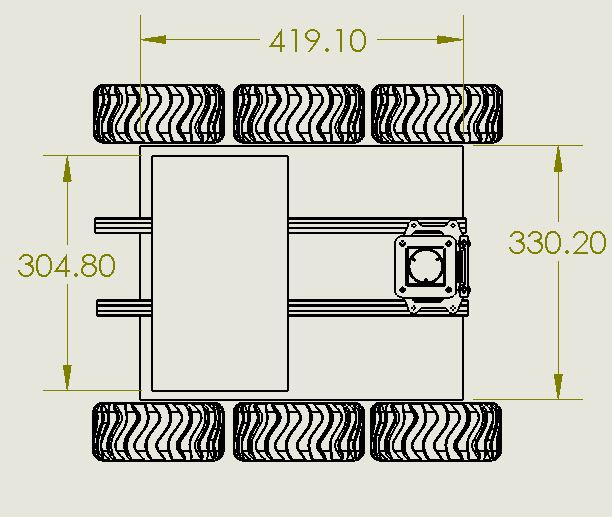
\includegraphics[width=1\textwidth]{GMMtop.jpg}
	\caption{Diagram of GMM.}
	\label{Figure 1:}
\end{figure}

\begin{figure}[h]
	\centering
	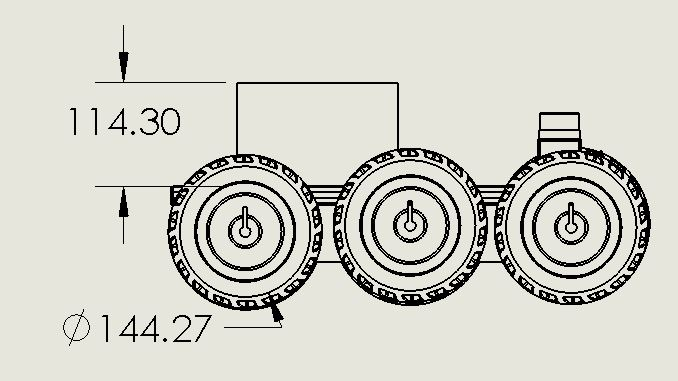
\includegraphics[width=1\textwidth]{GMMside.jpg}
	\caption{Diagram of GMM.}
	\label{Figure 1:}
\end{figure}
\begin{table}
\begin{tabular}{| l | l |}
 		\hline
 		Weight & 16 lb 7.9 oz  \\ \hline
 		Overall Height & 10" \\ \hline
 		Overall Length & 21" \\ \hline
 		Overall Width & 20.5"\\ \hline
	\end{tabular}
	\caption{GMM Specifications.}
\end{table}

\begin{figure}[h]
	\centering
	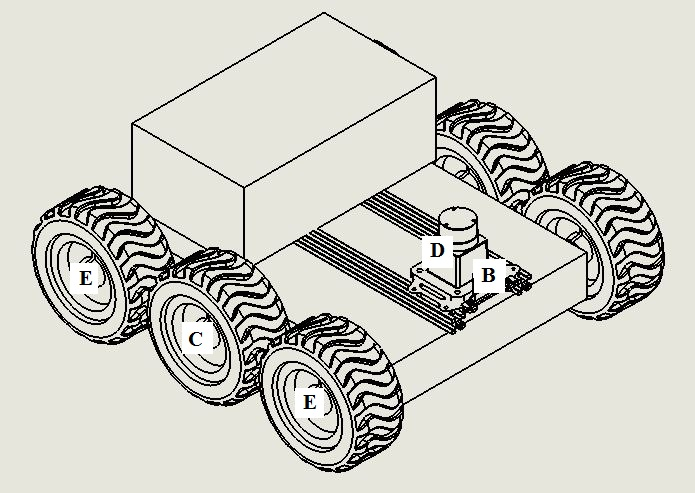
\includegraphics[width=1\textwidth]{GMMlabel.jpg}
	\caption{Diagram of GMM.}
	\label{Figure 1:}
\end{figure}

\begin{figure}[h]
	\centering
	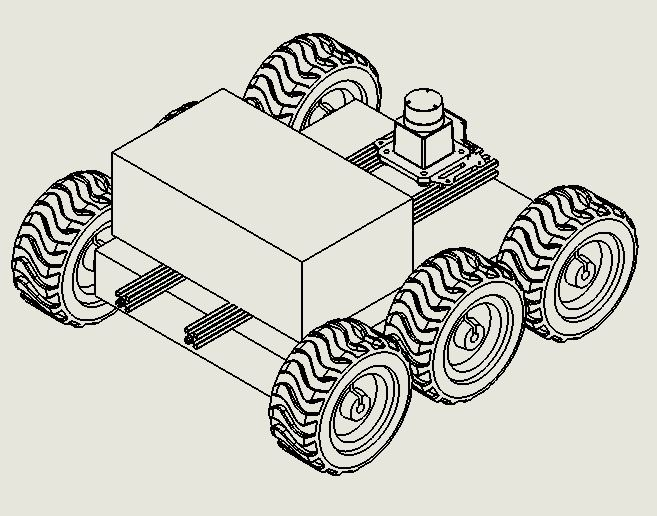
\includegraphics[width=1\textwidth]{gmmBehind.jpg}
	\caption{Diagram of GMM.}
	\label{Figure 1:}
\end{figure}


\begin{table}
\begin{tabular}{| l | p{3cm} | p{10cm} |}
 		\hline
 		Label & Component & Description \\ \hline 
 		A & Autopilot & RM48L952 and TM4C123GH6PZ processors\\ \hline
 		B & Camera & Support 5M video streaming, Focusing Range: 60cm to infinity\\ \hline
 		C & Encoders & 2.6 kHz sampling rate \\ \hline
 		D & LIDAR & Accuracy $\pm$30mm, Range 5600mm x 240$\degrees$, Scanning time 100ms/scan, Angular Resolution Step angle : approx. 0.36\\ \hline
 		E & Motors & No-Load Speed: 165 RPM, Max Torque: 680.5 oz-in.\\ \hline
 		F & Wifi & TP Link, Wireless Standard IEEE 802.11n, IEEE 802.11g, IEEE 802.11b\\ \hline
 		G & Odroid & Samsung Exynos5422 Cortex™-A15 2.0Ghz quad core and Cortex™-A7 quad core CPUs, LPDDR3 RAM at 933MHz \\ \hline
 
	\end{tabular}
	\caption{List of GMM major components.}
\end{table}

\chapter{Block Diagrams}
\section{Communication and Control Diagram}
\begin{figure}[h]
	\centering
	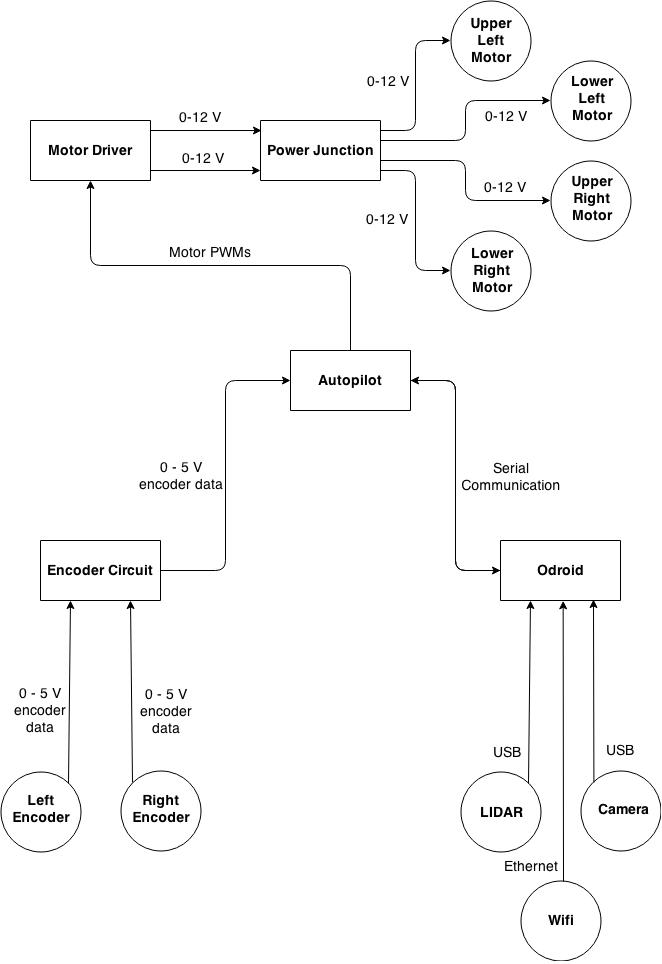
\includegraphics[width=0.8\textwidth]{commdiag.jpg}
	\caption{Diagram of communication connections.}
	\label{Figure 1:}
\end{figure}
\section{Power Diagram}
\begin{figure}[h]
	\centering
	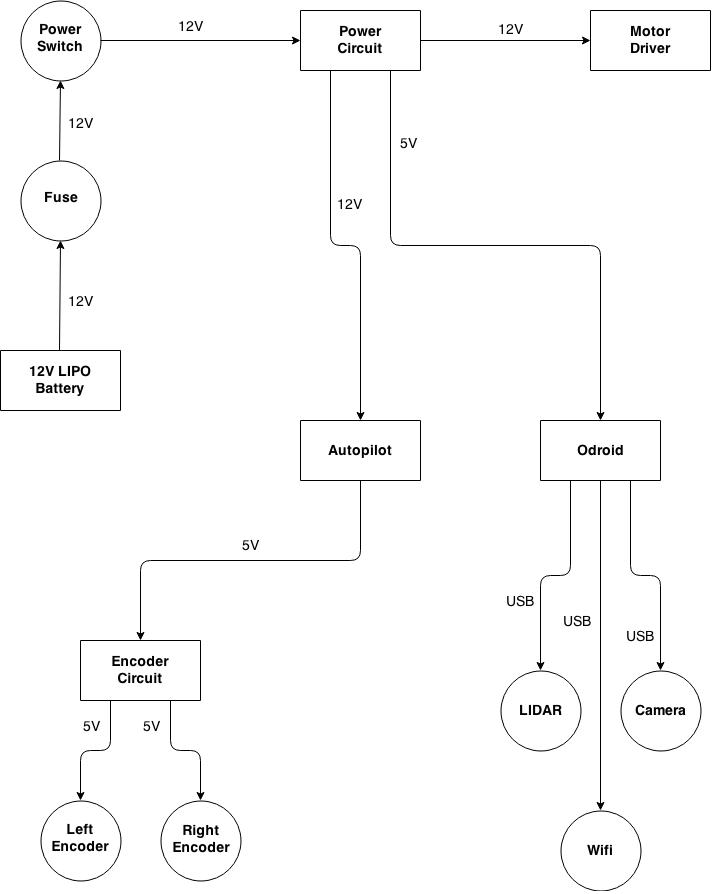
\includegraphics[width=0.8\textwidth]{powerdiag.jpg}
	\caption{Diagram of power connections.}
	\label{Figure 1:}
\end{figure}
\chapter{Connections}
\section{Autopilot}
Almost all connections to and from the autopilot, including power are done through the main 50 pin connector on the top of the autopilot. The serial connection to the Odroid is the only connection not make through the 50 pin connector but made through the JTAG on the back of the autopiot. The autopilot is connected to the encoders to provide 5V to power them as well as read the data from them through the ADC. Two PWMs are connected the motor driver to control the motors on the left and right side of the robot. A JTAG connector on the back of the Autopilot connects the SCI2 serial interface to the Odroid.

\begin{figure}[h]
	\centering
	\includegraphics[width=1\textwidth]{autopilot.jpg}
	\caption{50 pin Connector on the Autopilot}
	\label{Figure 1:}
\end{figure}

\begin{table}[h]
	\centering
	\begin{tabular}{| l |l | l |}
 		\hline
 		Pin Number & Function & GMM Connector \\ \hline 
 		1 & Input Power, Vin & 12V \\ \hline
 		7 & ADC & Encoders \\ \hline
 		8 & ADC & Encoders \\ \hline
 		15 & SCI RX & Debug \\ \hline
 		16 & SCI TX & Debug \\ \hline
 		17 & Regulated 5V & Encoders \\ \hline
 		35 & Motor PWM & PWM \\ \hline
 		36 & Motor PWM & PWM \\ \hline
 		2,?,?,? & GND & 12V, Encoders, Debug, PWM \\ \hline
 		All Others & See Autopilot manual & Not Used \\ \hline

	\end{tabular}
	\caption{Autopilot connections.}
\end{table}

\section{Encoder and Power Junction Circuit}
This circuit provides connections between the motor driver and the motors and the autopilot and the encoders. The power from the motor drivers is sent to both motors. The power from the autopilot is sent to both encoders and their data line is connected to the autopilot.
\begin{figure}[h]
	\centering
	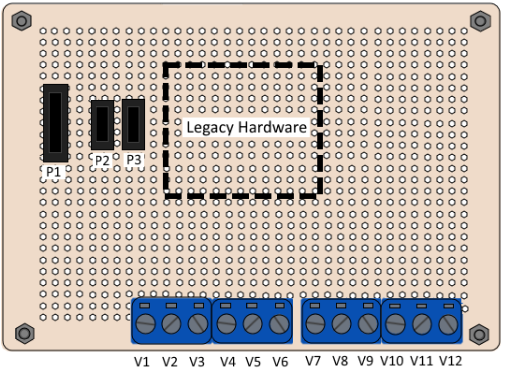
\includegraphics[width=1\textwidth]{encodercircuit2.jpg}
	\caption{Diagram of encoder and power junction circuit with connectors and voltage ports labeled.}
	\label{Figure 1:}
\end{figure}

\begin{table}[h]
	\centering
	\begin{tabular}{| l | l | l |}
 		\hline
 		Voltage Port & Voltage & Connected To \\ \hline 
 		V1 & A  & To upper left motor \\ \hline
 		V2 & B & To upper left motor \\ \hline
 		V3 & A & To lower left motor \\ \hline
 		V4 & B & To lower left motor \\ \hline
 		V5 & A & From motor driver \\ \hline
 		V6 & B & From motor driver \\ \hline
 		V7 & A & To upper right motor \\ \hline
 		V8 & B & To upper right motor \\ \hline
 		V9 & A & To lower right motor\\ \hline
 		V10 & B & To lower right motor \\ \hline
 		V11 & A & From motor driver \\ \hline
 		V12 & B & From motor driver \\ \hline
	\end{tabular}
	\caption{Encoder and power junction circuit connections.}
\end{table}

\begin{figure}[h]
	\centering
	\includegraphics[width=0.5\textwidth]{encoderports2.jpg}
	\caption{Diagram of encoder and power junction circuit with connectors and voltage ports labeled.}
	\label{Figure 1:}
\end{figure}
Port P1 is connected to the autopilot. It sends power to the encoders and receives their voltage signals, from both the left and right side encoders. Ports P3 and P2 are connected to the encoders, the signals are then send to the autopilot port and their power is connected to the power from the autopilot connector. Both the left and right encoder are connected in the same way, meaning the ports P2 and P3 have the same connections. Port P2 is connected to the right encoder and port P3 is connected to the left encoder.
 
\begin{table}[h]
	\centering
	\begin{tabular}{| l | l | l |}
 		\hline
 		Pin & Function & Value) \\ \hline 
 		1 & Right encoder voltage & 0 - 3.3V \\ \hline
 		2 & Left encoder voltage & 0 - 3.3V \\ \hline
 		3 & Encoder Vin & 3.3V \\ \hline
 		4 & GND & 0V \\ \hline
	\end{tabular}
	\caption{Port P1, connected to autopilot.}
\end{table}

\begin{table}[h]
	\centering
	\begin{tabular}{| l | l | l |}
 		\hline
 		Pin & Function & Value) \\ \hline 
 		1 & Encoder voltage & 0 - 3.3V \\ \hline
 		2 & Encoder Vin & 3.3V \\ \hline
 		3 & GND & 0V \\ \hline
	\end{tabular}
	\caption{Port P2 and P3, connected to encoders.}
\end{table}


\section{Motor Driver}
The motor driver receives PWM signals for the right and left side of the robot. It then outputs the corresponding voltage to send to the motors. These voltages are sent to the power junction circuit to give the same voltage to both right side motors and both left side motors.
\begin{figure}[h]
	\centering
	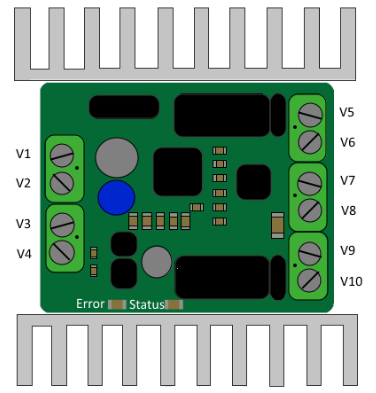
\includegraphics[width=0.6\textwidth]{motordriver2.jpg}
	\caption{Diagram motor driver with voltage ports labeled.}
	\label{Figure 1:}
\end{figure}
\begin{table}[h]
	\centering
	\begin{tabular}{| l | l | l |}
 		\hline
 		Voltage Port & Voltage & Connected To \\ \hline 
 		V1 & GND  & Autopilot \\ \hline
 		V2 & - & Unconnected \\ \hline
 		V3 & PWM & Autopilot \\ \hline
 		V4 & PWM & Autopilot \\ \hline
 		V5 & B for right side encoders & To power junction circuit \\ \hline
 		V6 & A for right side encoders & To power junction circuit \\ \hline
 		V7 & GND & From power circuit  \\ \hline
 		V8 & GND & From power circuit \\ \hline
 		V9 & A for left side encoders  & To power junction circuit\\ \hline
 		V10 & B for left side encoders & To lower right motor \\ \hline
	\end{tabular}
	\caption{Motor driver connections.}
\end{table}

\section{Odroid}
All Odroid connections, except for its power source are made by USB on the front side of the odroid. The power connects with a round plug into the backside. The Odroid gets data from the camera, lidar, and autopilot. The Odroid also sends data to the autopilot through serial connection, to send movement commands to the autopilot which in turn controls the motors. 
\begin{figure}[h]
	\centering
	\includegraphics[width=1\textwidth]{odroidfront.png}
	\caption{Diagram of labeled Odroid connection ports, front of odroid.}
	\label{Figure 1:}
\end{figure}
\begin{table}[h]
	\centering
	\begin{tabular}{| l | l | l |}
 		\hline
 		Port & Type & Current Use \\ \hline 
 		P1 & 10/100 Ethernet & Wifi, TP-LINK \\ \hline
 		P2 & USB 2.0 Host & Wifi, TP-LINK power \\ \hline
 		P3 & USB 2.0 Host & Autopilot SCI \\ \hline
 		P4 & USB 2.0 Host & Camera \\ \hline
 		P5 & USB 2.0 Host & Not used \\ \hline
 		P6 & Display Port & Not used\\ \hline
	\end{tabular}
	\caption{Odroid front connections.}
\end{table}
\begin{figure}[h]
	\centering
	\includegraphics[width=1\textwidth]{odroidback2.jpg}
	\caption{Diagram of labeled Odroid connection ports, back of odroid.}
	\label{Figure 1:}
\end{figure}
\begin{table}[h]
	\centering
	\begin{tabular}{| l | l | l |}
 		\hline
 		Port & Type & Current Use \\ \hline 
 		P1 & DC Jack 5V, 4A & 5V power from Autopilot \\ \hline
 		P2 & USB 3.0 Host & Camera \\ \hline
 		P3 & USB 3.0 OTG & Not used \\ \hline
 		P4 & Micro SD Slot & Not used \\ \hline
 		P5 & Micro HDMI & Not used \\ \hline
 		P6 & Headphone Jack & Not used \\ \hline
	\end{tabular}
	\caption{Odroid back connections.}
\end{table}

\section{Power Circuit}
This board takes 12V input from the battery and splits it to other parts of the robot. The autopilot and motor drivers both receive 12V from this board and the Odroid recieves a regulated 5V.
\begin{figure}[h]
	\centering
	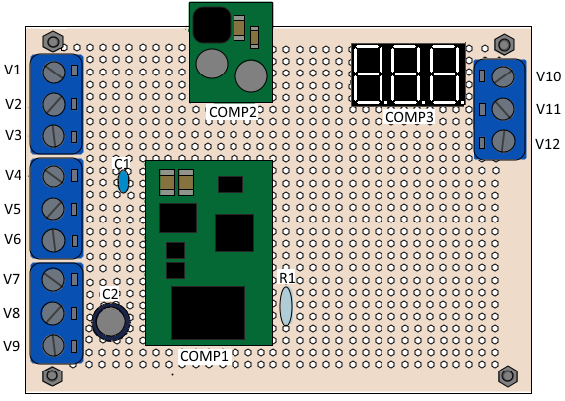
\includegraphics[width=0.8\textwidth]{powercircuit2.jpg}
	\caption{Diagram of power circuit with voltage ports and parts labeled.}
	\label{Figure 1:}
\end{figure}
\begin{table}[h]
	\centering
	\begin{tabular}{| l | l |}
 		\hline
 		Component & Function \\ \hline 
 		COMP1 & 6V Regulator \\ \hline
 		COMP2 & 5V Regulator  \\ \hline
 		COMP3 & Voltage Monitor  \\ \hline
	\end{tabular}
	\caption{List of components on power circuit.}
\end{table}
\begin{table}[h]
	\centering
	\begin{tabular}{| l | l | l |}
 		\hline
 		Voltage Port & Voltage & Connected To \\ \hline 
 		V1 & 12V & To motor driver \\ \hline
 		V2 & GND & To motor driver \\ \hline
 		V3 & 12V & To autopilot \\ \hline
 		V4 & GND & To autopilot \\ \hline
 		V5 & 5V V & To odroid \\ \hline
 		V6 & GND & To odroid \\ \hline
 		V7 & 6V & Unused \\ \hline
 		V8 & 6V V & Unused \\ \hline
 		V9 & GND & Unused\\ \hline
 		V10 & 12V & From switch \\ \hline
 		V11 & GND V & From switch \\ \hline
 		V12 & Unconnected & Unused \\ \hline
	\end{tabular}
	\caption{Odroid front connections.}
\end{table}
\chapter{ADC and DAC Filters}
\begin{figure}[h]
	\centering
	\includegraphics[width=0.6\textwidth]{filter.jpg}
	\caption{Diagram of filter circuit.}
	\label{Figure 1:}
\end{figure}
\begin{table}[h]
	\centering
	\begin{tabular}{| l | l | l |}
 		\hline
 		Component & Autopilot Component Name & Value \\ \hline 
 		R1 & Zix4 & 1.1k ohm \\ \hline
 		R2 & Zix3 & 1.1k ohm \\ \hline
 		R3 & Zix1 & 2.2k ohm \\ \hline
 		R4 & Zmx1 & 15.9k ohm \\ \hline
 		C1 & Zix2 V & 1 microF \\ \hline
 		C2 & Zix5 & 115nF \\ \hline
 		C3 & Zmx2 & 1.31micrpF \\ \hline
 	
	\end{tabular}
	\caption{Filter component values.}
\end{table}

Gain = 0.5 \par
Cutoff frequency = 132 Hz \par
Dampening Coefficient = 0.1527 \par
Cutoff frequency of voltage offset = 10 Hz \par

\chapter{Part List}

A Autopilot \par
\setlength{\parindent}{5ex}
Version 2.3.1 \par
See Autopilot Documentation for more information \par
\noindent
B Battery \par
12V LIPO Battery 3S \par
Lab made 3 series packs	\par
\noindent
C Camera \par
Leopard Imaging LI-OV5640-USB-72 \par
https://www.leopardimaging.com/LI-OV5640-USB-72.html \par
\noindent
D Encoders \par
US Digital MA3 Miniature Absolute Magnetic Shaft Encoder \par
http://www.usdigital.com/products/encoders/absolute/rotary/shaft/MA3 \par	
\noindent
E Encoder and Power Junction Circuit \par
new part coming soon! \par
\noindent
F LIDAR \par
Hokuyo URG-04LX-UG01 Scanning Laser Rangefinder \par
%https://www.hokuyo-aut.jp/02sensor/07scanner/urg_04lx_ug01.html	\par
\noindent
G Motors \par
165 RPM HD Precision Planetary Gear Motor \par
%https://www.servocity.com/html/165_rpm_hd_precision_planetary.html#.VOoI0PnF9yy \par
\noindent	
H Motor Drivers \par
Sabertooth 2x12 \par
https://www.dimensionengineering.com/datasheets/Sabertooth2x12.pdf \par
\noindent	
I Odroid \par
Odroid XU3 \par
%http://www.hardkernel.com/main/products/prdt_info.php?g_code=G140448267127 \par
\noindent	
J Power Circuit \par
5V Regulator \par
\setlength{\parindent}{10ex}
5V, 5A step-down voltage regulator D24V50F5 \par
https://www.pololu.com/product/2851 \par
\setlength{\parindent}{5ex}
6V Regulator \par
\setlength{\parindent}{10ex}
Texas Instruments PTN78020WAH \par
http://www.digikey.com/product-detail/en/PTN78020WAH/296-20515-ND/717485 \par
\noindent		 
Fuse \par
\setlength{\parindent}{5ex}
10A \par 
\noindent	
Fuse Holder \par
30A max \par
\end{document}